\documentclass[10pt, oneside]{article} 
\usepackage{amsmath, amsthm, amssymb, calrsfs, wasysym, verbatim, bbm, color, graphics, graphicx, tocloft, subcaption, blindtext, hyperref, listings}
\usepackage[margin=1in]{geometry}

\title{Security \& Cryptography Assignment 1}
\author{Anna Visman 6351115}
\date{01/12/2025}

\begin{document}

\maketitle

\section{Historical Ciphers}

\begin{itemize}
    \item[a)] This ciphertext is made using the Caesar cipher with a shift(key) of 5. The plaintext is: 
    
    To be, or not to be, that is the question: Whether ’tis nobler in the mind to
    suffer The slings and arrows of outrageous fortune, Or to take arms against a
    sea of troubles And by opposing end them. To die—to sleep, No more; and by a sleep
    to say we end The heart-ache and the thousand natural shocks That flesh is
    heir to: ’tis a consummation Devoutly to be wish’d.

    \item[b)] This cipher is made using the Vigenère cipher with the key "oppenheimer". The plaintext is:
    
    Reveal Thy Self; what awful Form art Thou? I worship Thee! Have mercy, God
    supreme! Thine inner Being I am fain to know; This Thy forth-streaming
    Life bewilders me.
    Time am I, laying desolate the world, Made manifest on earth to slay mankind!
    Not one of all these warriors ranged for strife Escapeth death; thou shalt
    alone survive.
    Therefore stand up! win for thyself renown, Conquer thy foes, enjoy the wealth
    filled realm, By Me they are already overcome, Be thou the outward cause,
    left-handed one. Drona and Bhîshma and Jayadratha, Karna, and all the other
    warriors here, Are slain by Me. Destroy them fearlessly. Fight! thou shalt
    crush thy rivals in the field.
    Sanjaya said: Having heard these words of Keshava, he who weareth a diadem,
    with joined palms, quaking and prostrating himself, spake again to Kri-
     shna, stammering with fear, casting down his face.
            
    \item[c)] The code for the cipher in part a) can be found in appendix \ref{caesar}. A proof of the resulting key and plaintext can be found in appendix \ref{caesarproof}.
\end{itemize}

\section{Number Theory and Elliptic Curve}
\begin{itemize}
    \item[a)] $x \equiv 13^{\frac{1}{7}} \mod 119$ is equivalent to $x^7 \equiv 13 \mod 119$ 
    \item[b)] $F: y^2 = x^3 - 2x + 2 \mod 71, P=(1,1), Q = (4,49)$, so $a = -2, b = 2, p = 71$.
    
    $2P =(x_3, y_3):$ \\
    $\lambda = \frac{3\cdot x_1^2 + a}{2y_1} = \frac{3 \cdot 1^2 -2 }{2 \cdot 1} = \frac{1}{2} = 1 \cdot 2^{-1} \mod 71$ \\

    Find the modular inverse of $2 \mod 71$: \\
    $2k \equiv 1 \mod 71$. Clearly, $2\cdot 36 = 72 \equiv 1 \mod 71$. So, $2^{-1} = 36$. Then $\lambda = 36 \pmod{71}$.\\
    
    $x_3 = \lambda^2 - 2x_1 = 36^2 - 2 \cdot 1 = 1294 \mod 71 =  16 \pmod{71}$ \\
    $y_3 = \lambda(x_1 - x_3) - y_1 = 36(1-16) - 1 = 36 \cdot -15 - 1 = -541 \mod 71= -541 + 8\cdot 71 \mod 71 = 27 \pmod{71}$ \\
    
    So, $2P = (16, 27)$. \\

    $P + Q = (x_3, y_3):$\\
    $\lambda = \frac{y_2 - y_1}{x_2 - x_1} = \frac{49 - 1}{4 - 1} = \frac{48}{3} = 16 \mod 71$\\

    $x_3 = \lambda^2 - x_1 - x_2 = 16^2 - 1 - 4 = 256 - 5 = 251 \mod 71 =  38 \pmod{71}$ \\
    $y_3 = \lambda(x_1 - x_3) - y_1 = 16(1-38) - 1 = 16 - 609 \mod 71 = -593 \mod 71 = -593 + 9 \cdot 71 \mod 71= 46 \pmod{71}$ \\
    So, $P + Q = (38, 46)$.
\end{itemize}

\section{Information Theoretic Security}

\begin{itemize}
    \item[a)] To avoid hand calculations, I coded the formulas required for this exercise. My code can be found in appendix \ref{3a-code}. \\
    
    First we calculate the probability of each cipher text occuring usings the formula:
    \[ p(C=c) = p(P=m) \cdot p(C=c | P=m) \]

    $P(C=1) = p(K=k_1) \cdot p(P=b) +  p(K=k_2) \cdot p(P=c) + p(K=k_3) \cdot p(P=d) + p(K=k_4) \cdot p(P=a) = \frac{1}{5}\cdot \frac{4}{15} +  \frac{3}{10}\cdot \frac{1}{5} +  \frac{1}{5}\cdot \frac{1}{5} +  \frac{3}{10}\cdot \frac{1}{3} = 0.25\bar{3}$

    Repeating this for the other ciphertexts gives:

    $P(C=2) = 0.25\bar{3}$ 

    $P(C=3) = 0.24\bar{6}$

    $P(C=4) = 0.24\bar{6}$

    Then, we calculate the probability of each cipher text occuring given the plaintext and key distributions using the encryption schema:

    \[
    p(C=c) = \sum_{k: c\in \mathbb{C}(k)} p(K=k)\cdot p(P=d_k(c))
    \]

    \[
\begin{aligned}
    &P(C = 1 \mid P = a) = 0.3, \quad P(C = 2 \mid P = a) = 0.3, \quad P(C = 3 \mid P = a) = 0.2, \quad P(C = 4 \mid P = a) = 0.2, \\
    &P(C = 1 \mid P = b) = 0.2, \quad P(C = 2 \mid P = b) = 0.2, \quad P(C = 3 \mid P = b) = 0.3, \quad P(C = 4 \mid P = b) = 0.3, \\
    &P(C = 1 \mid P = c) = 0.3, \quad P(C = 2 \mid P = c) = 0.3, \quad P(C = 3 \mid P = c) = 0.2, \quad P(C = 4 \mid P = c) = 0.2, \\
    &P(C = 1 \mid P = d) = 0.2, \quad P(C = 2 \mid P = d) = 0.2, \quad P(C = 3 \mid P = d) = 0.3, \quad P(C = 4 \mid P = d) = 0.3.
    \end{aligned}
    \]


    Finally, we can calculate the probability of each plaintext conditioned on each ciphertext occurrence (see code in appendix):
    \[
    p(P=m |C=c) = \frac{p(P=m) \cdot p(C=c | P=m)}{p(C=c)}
    \]

    \[
\begin{aligned}
    &P(P = a \mid C = 1) = 0.395, \quad P(P = a \mid C = 2) = 0.395, \quad P(P = a \mid C = 3) = 0.270, \quad P(P = a \mid C = 4) = 0.270, \\
    &P(P = b \mid C = 1) = 0.211, \quad P(P = b \mid C = 2) = 0.211, \quad P(P = b \mid C = 3) = 0.324, \quad P(P = b \mid C = 4) = 0.324, \\
    &P(P = c \mid C = 1) = 0.237, \quad P(P = c \mid C = 2) = 0.237, \quad P(P = c \mid C = 3) = 0.162, \quad P(P = c \mid C = 4) = 0.162, \\
    &P(P = d \mid C = 1) = 0.158, \quad P(P = d \mid C = 2) = 0.158, \quad P(P = d \mid C = 3) = 0.243, \quad P(P = d \mid C = 4) = 0.243.
\end{aligned}
\]



    \item[b)]We use the formula for conditional entropy from the slides: 
    \[H(M \mid C) = \sum_{c} p(C = c) \cdot H(M \mid C = c) 
    = - \sum_{m} \sum_{c} p(C = c) \cdot p(M = m \mid C = c) \cdot \log_2 p(M = m \mid C = c). \]    

    to write the code in appendix \ref{3b-code} and calculate the value. We find:
    \[H(M \mid C) \approx 0.458\] 
    \item[c)] A cryptosystem has perfect secrecy if \[ p(P=m | C=c) = p(P=m) \] for all plain texts $m$ and ciphertexts $c$. It can be easily seen that this condition is already violated for $P=a$ with $p(P=a) = \frac{1}{3}$. So, the system does not have perfect secrecy. 

\end{itemize}


\appendix

\section{Code}
This section lists the code written to help solve exercises 1 and 3. 
\subsubsection{Exercise 1c:}

\textbf{Caesar cipher:} \label{caesar}
\begin{lstlisting}[language=Python]
# works only on letters 'a' to 'z'
# shift using unicode values
def cshift(text, shift):
    result = []
    for char in text:
        if char.isalpha():
            if char.islower():
                result.append(chr((ord(char) - 97 + shift) % 26 + 97))
            else:
                result.append(chr((ord(char) - 65 + shift) % 26 + 65))
        else:
            result.append(char)
    return ''.join(result)

def shiftback(text, shift):
    return cshift(text, -shift)

with open('cipher.txt') as f:
    cipher = f.read().strip()

for i in range(26):
    print(i, shiftback(cipher, i))
\end{lstlisting}

\subsubsection{Exercise 3a:}
\label{3a-code}
\begin{lstlisting}[language=Python]
M = [1/3, 4/15, 1/5, 1/5]
K = [1/5, 3/10, 1/5, 3/10]
    
m = ['a', 'b', 'c', 'd']
    
scheme = [
    [3, 1, 4, 2],
    [2, 4, 1, 3],
    [4, 2, 3, 1],
    [1, 3, 2, 4]
]

def prob_ciper(cipher, M, K, scheme):
    rows, cols = len(scheme), len(scheme[0])

    total = 0
    for i in range(rows):
        for j in range(cols):
            if scheme[i][j] == cipher:
                total+= M[i] * K[j]

    return total


for i in range(4):
    print(f"P(C={i+1}) =", prob_ciper(i+1, M, K, scheme))

def prob_cipher_given_plain(cipher, plain, K, scheme):
    rows, cols = len(scheme), len(scheme[0])

    total = 0

    col = ord(plain) - ord('a')

    # get only the column col
    col = [scheme[i][col] for i in range(rows)]

    for c in col:
        if c == cipher:
            total+= K[col.index(c)]

    return total

for char in m:
    for i in range(4):
        print(f"P(C={i+1}|P={char}) =", 
            prob_cipher_given_plain(i+1, char, K, scheme))

def prob_plain_given_cipher(plain, cipher, M, scheme):
    rows, cols = len(scheme), len(scheme[0])
    
    total = 0
    
    p = ord(plain) - ord('a')
    
    prob = M[p]*prob_cipher_given_plain(cipher, plain, K, scheme)/
        prob_ciper(cipher, M, K, scheme)
    
    return prob
    
for char in m:
    for i in range(4):
        print(f"P(P={char}|C={i+1}) =", 
            prob_plain_given_cipher(char, i+1, M, scheme))
\end{lstlisting}

\subsubsection{Exercise 3b:}
\label{3b-code}
\begin{lstlisting}[language=Python]

import math

def conditional_entropy(M, K, scheme, msg):
    m_total = 1
    for char in msg:
        c_total = 0
        for i in range(4):
            pc = prob_ciper(i+1, M, K, scheme)
            ppc = prob_plain_given_cipher(char, i+1, M, scheme)
    
            c_total += (pc * ppc * math.log(ppc, 2))
    
        m_total *= c_total
    
    return -1*m_total
\end{lstlisting}

\section{Proofs}

\begin{figure}[h!]
    \centering
    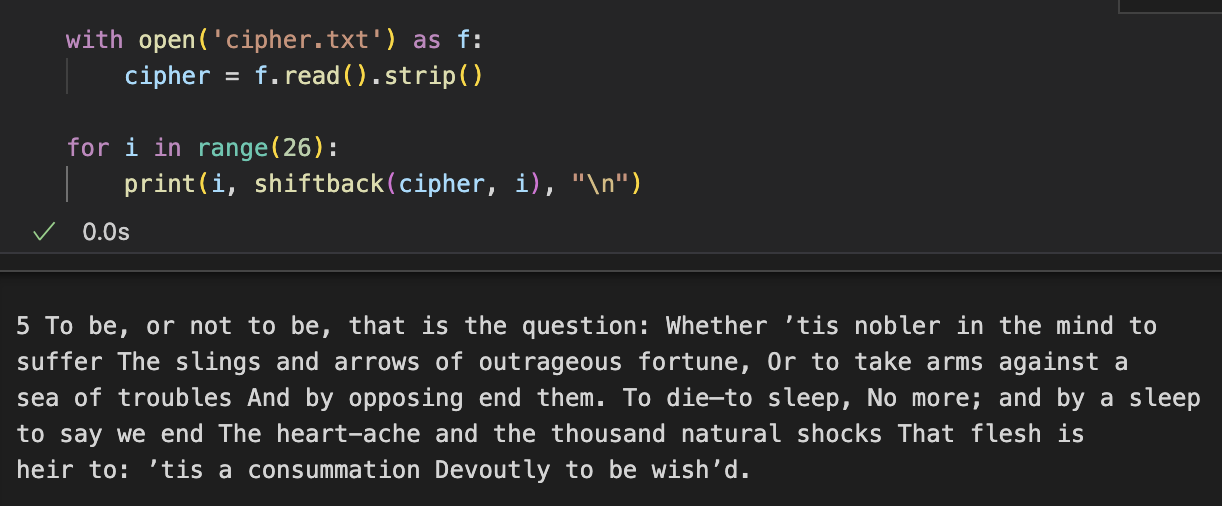
\includegraphics[scale=0.5]{img/caeser.png}
    \caption{Proof of code finding the plaintext using a shift of 5.}
    \label{caesarproof}
\end{figure}



\end{document}